\section{Résultats}

\subsection{Extraction du SOS et du EOS}

\`A partir des profils temporels de NDVI obtenus par les 2 méthodes de lissage (HANTS et Whittaker), nous avons extrait le SOS et le EOS respectivement avec les seuils de 10, 20, 30 puis 50\% avant le MAX et 50, 60, 70 puis 80\% après le MAX. Nous avons calculé ensuite pour chacune des parcelles terrain, les écarts en nombre de jours entre les dates de semis et les SOS extraits puis entre les dates de récolte et les EOS estimés. En considérant ces écarts par sytème de culture, nous avons calculé 2 indicateurs statistiques : la racine carrée de l'erreur quadratique moyenne ou \acrshort{rmse} qui est un indicateur d'écart entre valeurs observées et valeurs prédites et le coefficient de variation ou \acrshort{cv} qui mesure la dispersion autour la moyenne. 

\paragraph{SOS et évaluation des dates de semis}

La distribution des écarts entre les dates de semis observées et les SOS extraits par système de culture et méthode de lissage est illustrée sur la \cref{fig-sosboxplot}. Globalement, les parcelles d'arachide mixte montrent les variabilités les plus faibles entre les écarts calculés (moins de 15 jours d'écart au maximum, seuils et méthodes de lissage confondues) suivies des parcelles de mil pur (moins de 20 jours d'écart au maximum, seuils et méthodes de lissage confondues) et des parcelles de mil mixte qui présentent les variabilités les plus fortes (près de 60 jours d'écart avec les SOS estimés par HANTS pour un seuil de 10\%). En analysant la distribution des écarts par méthode de lissage, nous remarquons que pour l'ensemble des systèmes de culture et presque pour tous les seuils, la plage des écarts obtenus avec les SOS estimés par HANTS est toujours plus importante que celle des écarts obtenus avec les SOS extraits par la méthode de Whittaker. Ceci semble indiquer que la méthode de lissage de Whittaker soit plus appropriée pour estimer le timing du démarrage de croissance de la végétation. L'analyse de la distribution des écarts en fonction du seuil d'extraction du SOS montre quant à elle une certaine tendance à la réduction de la variabilité des écarts quand le seuil d'extraction s'accroit, méthodes de lissage et systèmes de culture confondus à l'exception du mil pur. Cependant, cette tendance est à relativiser au vu de l'apparition de valeurs aberrantes à mesure que le seuil d'extraction du SOS augmente et d'autant plus que les écarts entre dates de semis et SOS estimés s'accroissent également. En effet, il est tout à fait logique que ces écarts s'accroissent quand le seuil d'extraction du SOS augmente puisque l'amplitude du NDVI avant le MAX est proportionnelle au temps mais cela finit par ne plus être réaliste vis-à-vis du temps de germination des semences. Ainsi, si le seuil de 10\% a tendance à extraire des SOS précoces (écarts négatifs pour certaines parcelles d'arachide et mil mixtes), le seuil de 50\% les extrait tardivement (40 à 60 jours après les dates de semis). Sur la \cref{fig-sos-rmse-cv}, nous avons représenté le RMSE entre les dates de semis et SOS estimés en fonction du coefficient de variation (CV) de leurs écarts, par système de culture et méthode de lissage. Nous remarquons que quelque soit le système de culture et la méthode de lissage, plus le seuil d'extraction augmente, plus le RMSE est grand ce qui rejoint l'analyse sur la distribution des écarts en fonction du seuil d'extraction puisque ce dernier est un indicateur d'écart. Par contre, deux valeurs du coefficient de variation posent question : il s'agit de -233\% (seuil de 10\% avec la méthode de Whittaker pour l'arachide mixte) et 342\% (seuil de 10\% avec HANTS pour le mil mixte). Après vériication, il s'agit de cas où l'écart type est supérieure à une moyenne très petite (négative et positive respectivement) de 0. Ceci vient confirmer que les SOS extraits avec le seuil de 10\%





\begin{figure}[htbp]
 \begin{center}
  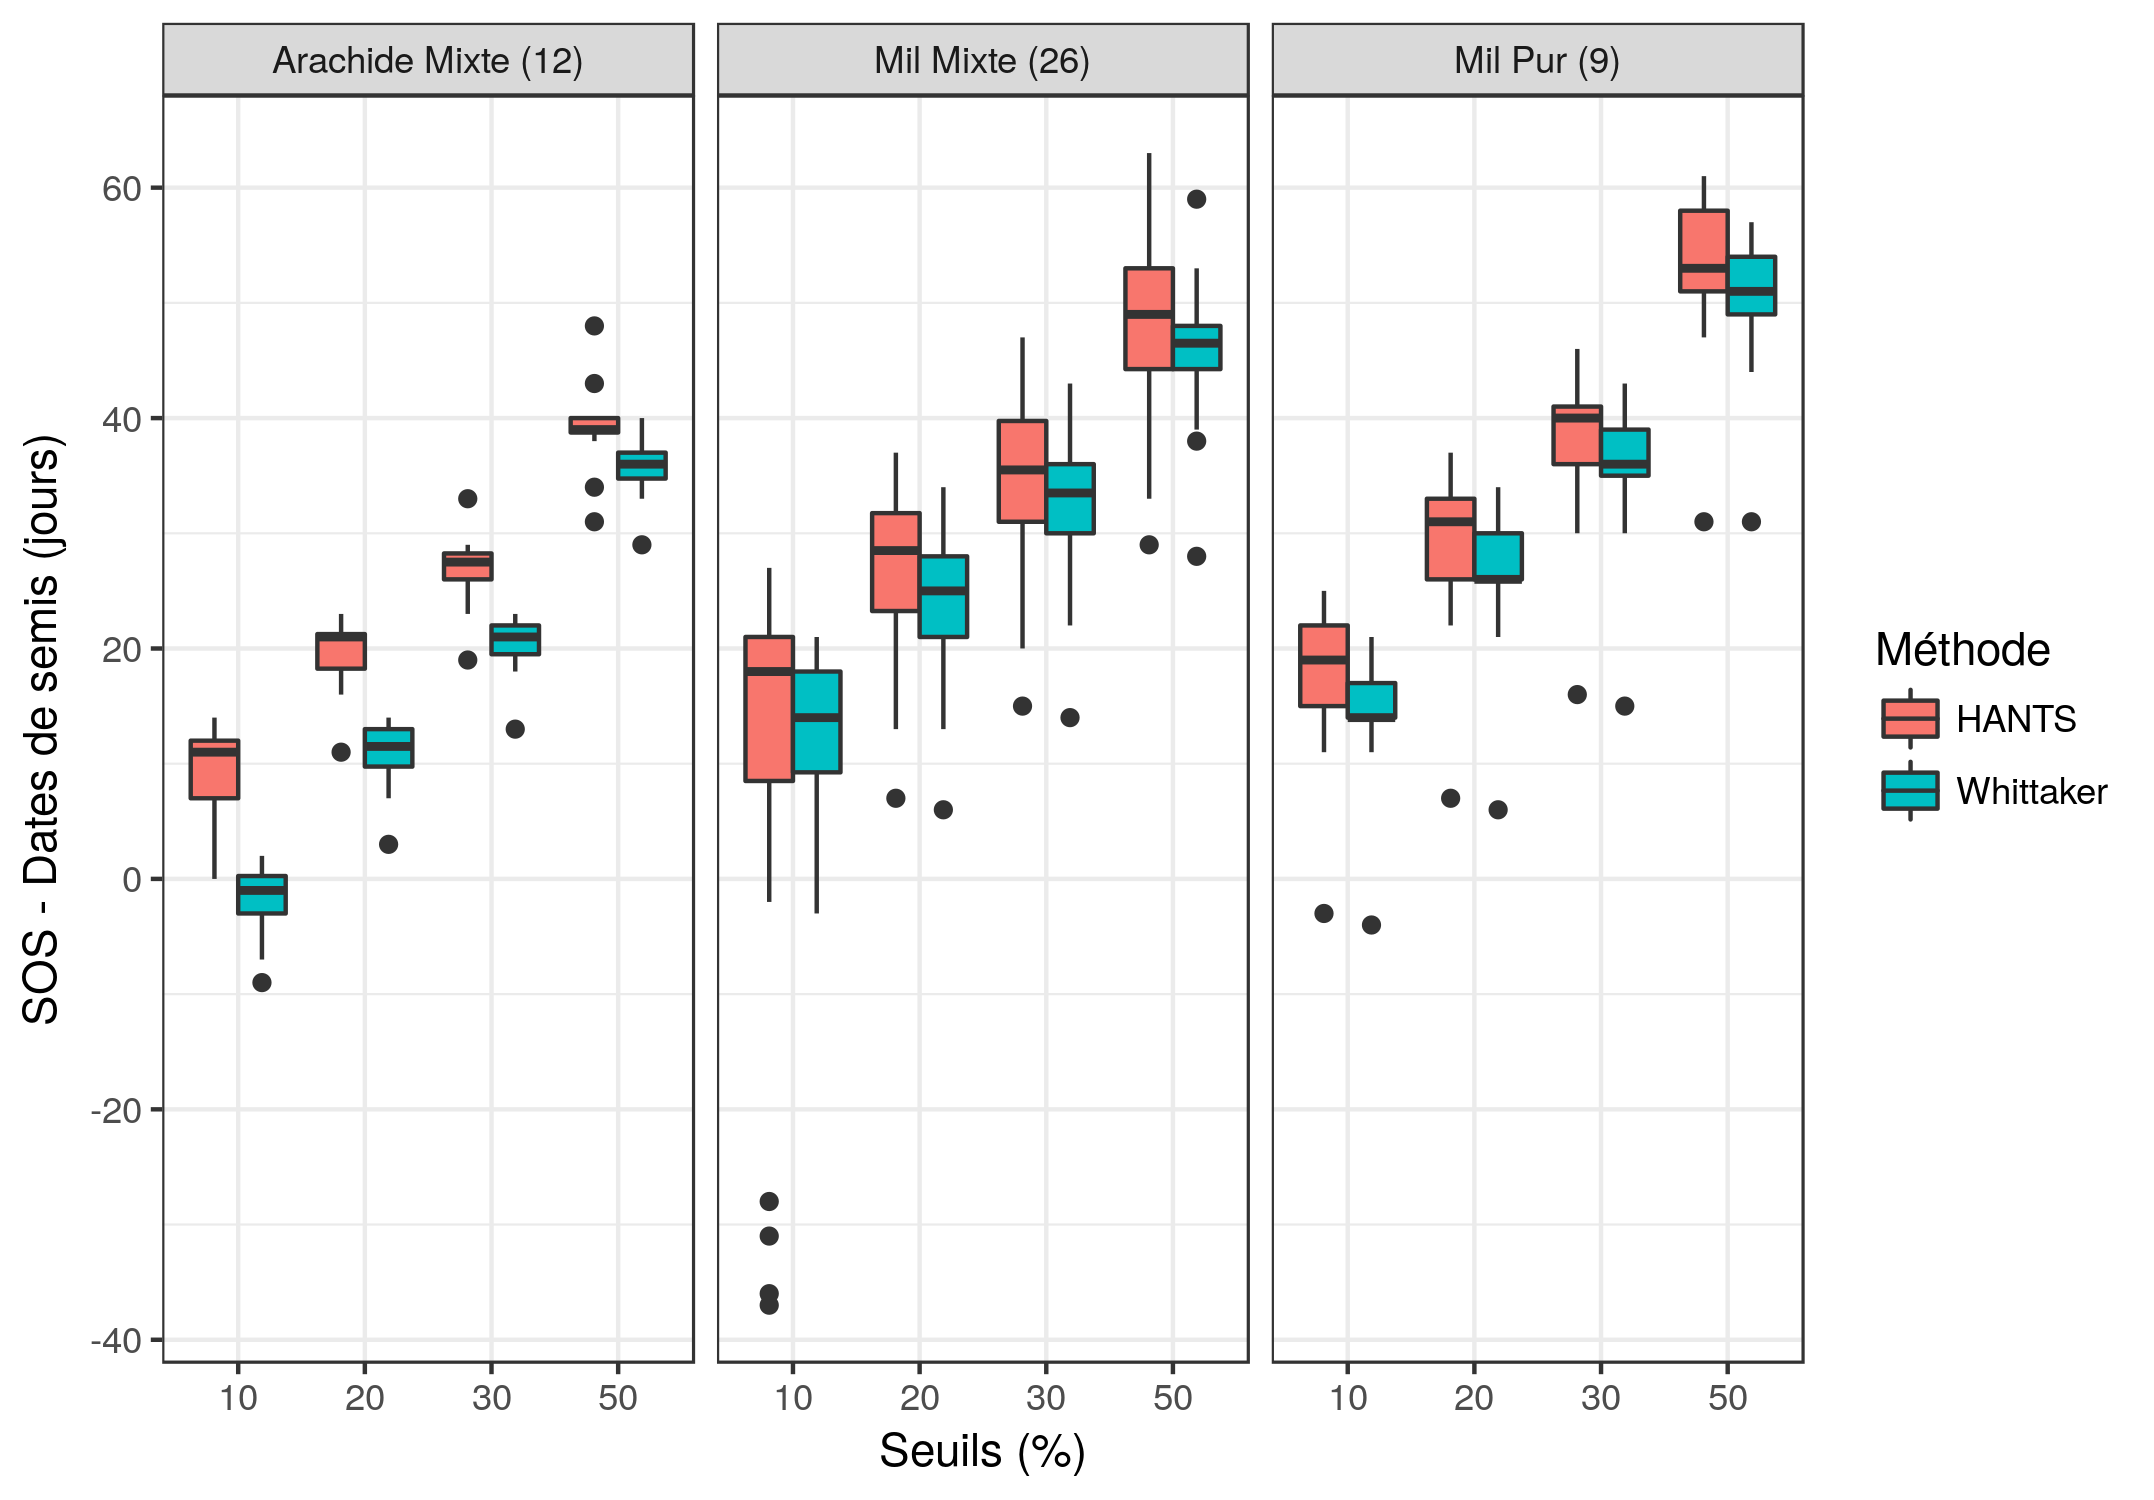
\includegraphics[scale=0.7]{resultats_discussions/SOS_Boxplot.png} 
 \end{center}
 \caption[Distribution des écarts entre SOS et dates de semis]{Boîtes à moustaches illustrant la distribution des écarts entre SOS estimés et dates de semis en fonction des systèmes de culture et des méthodes de lissage (\emph{Le nombre de parcelles est indiqué à la suite du système de culture})}
 \label{fig-sosboxplot}
\end{figure}

\begin{figure}[htbp]
 \begin{center}
  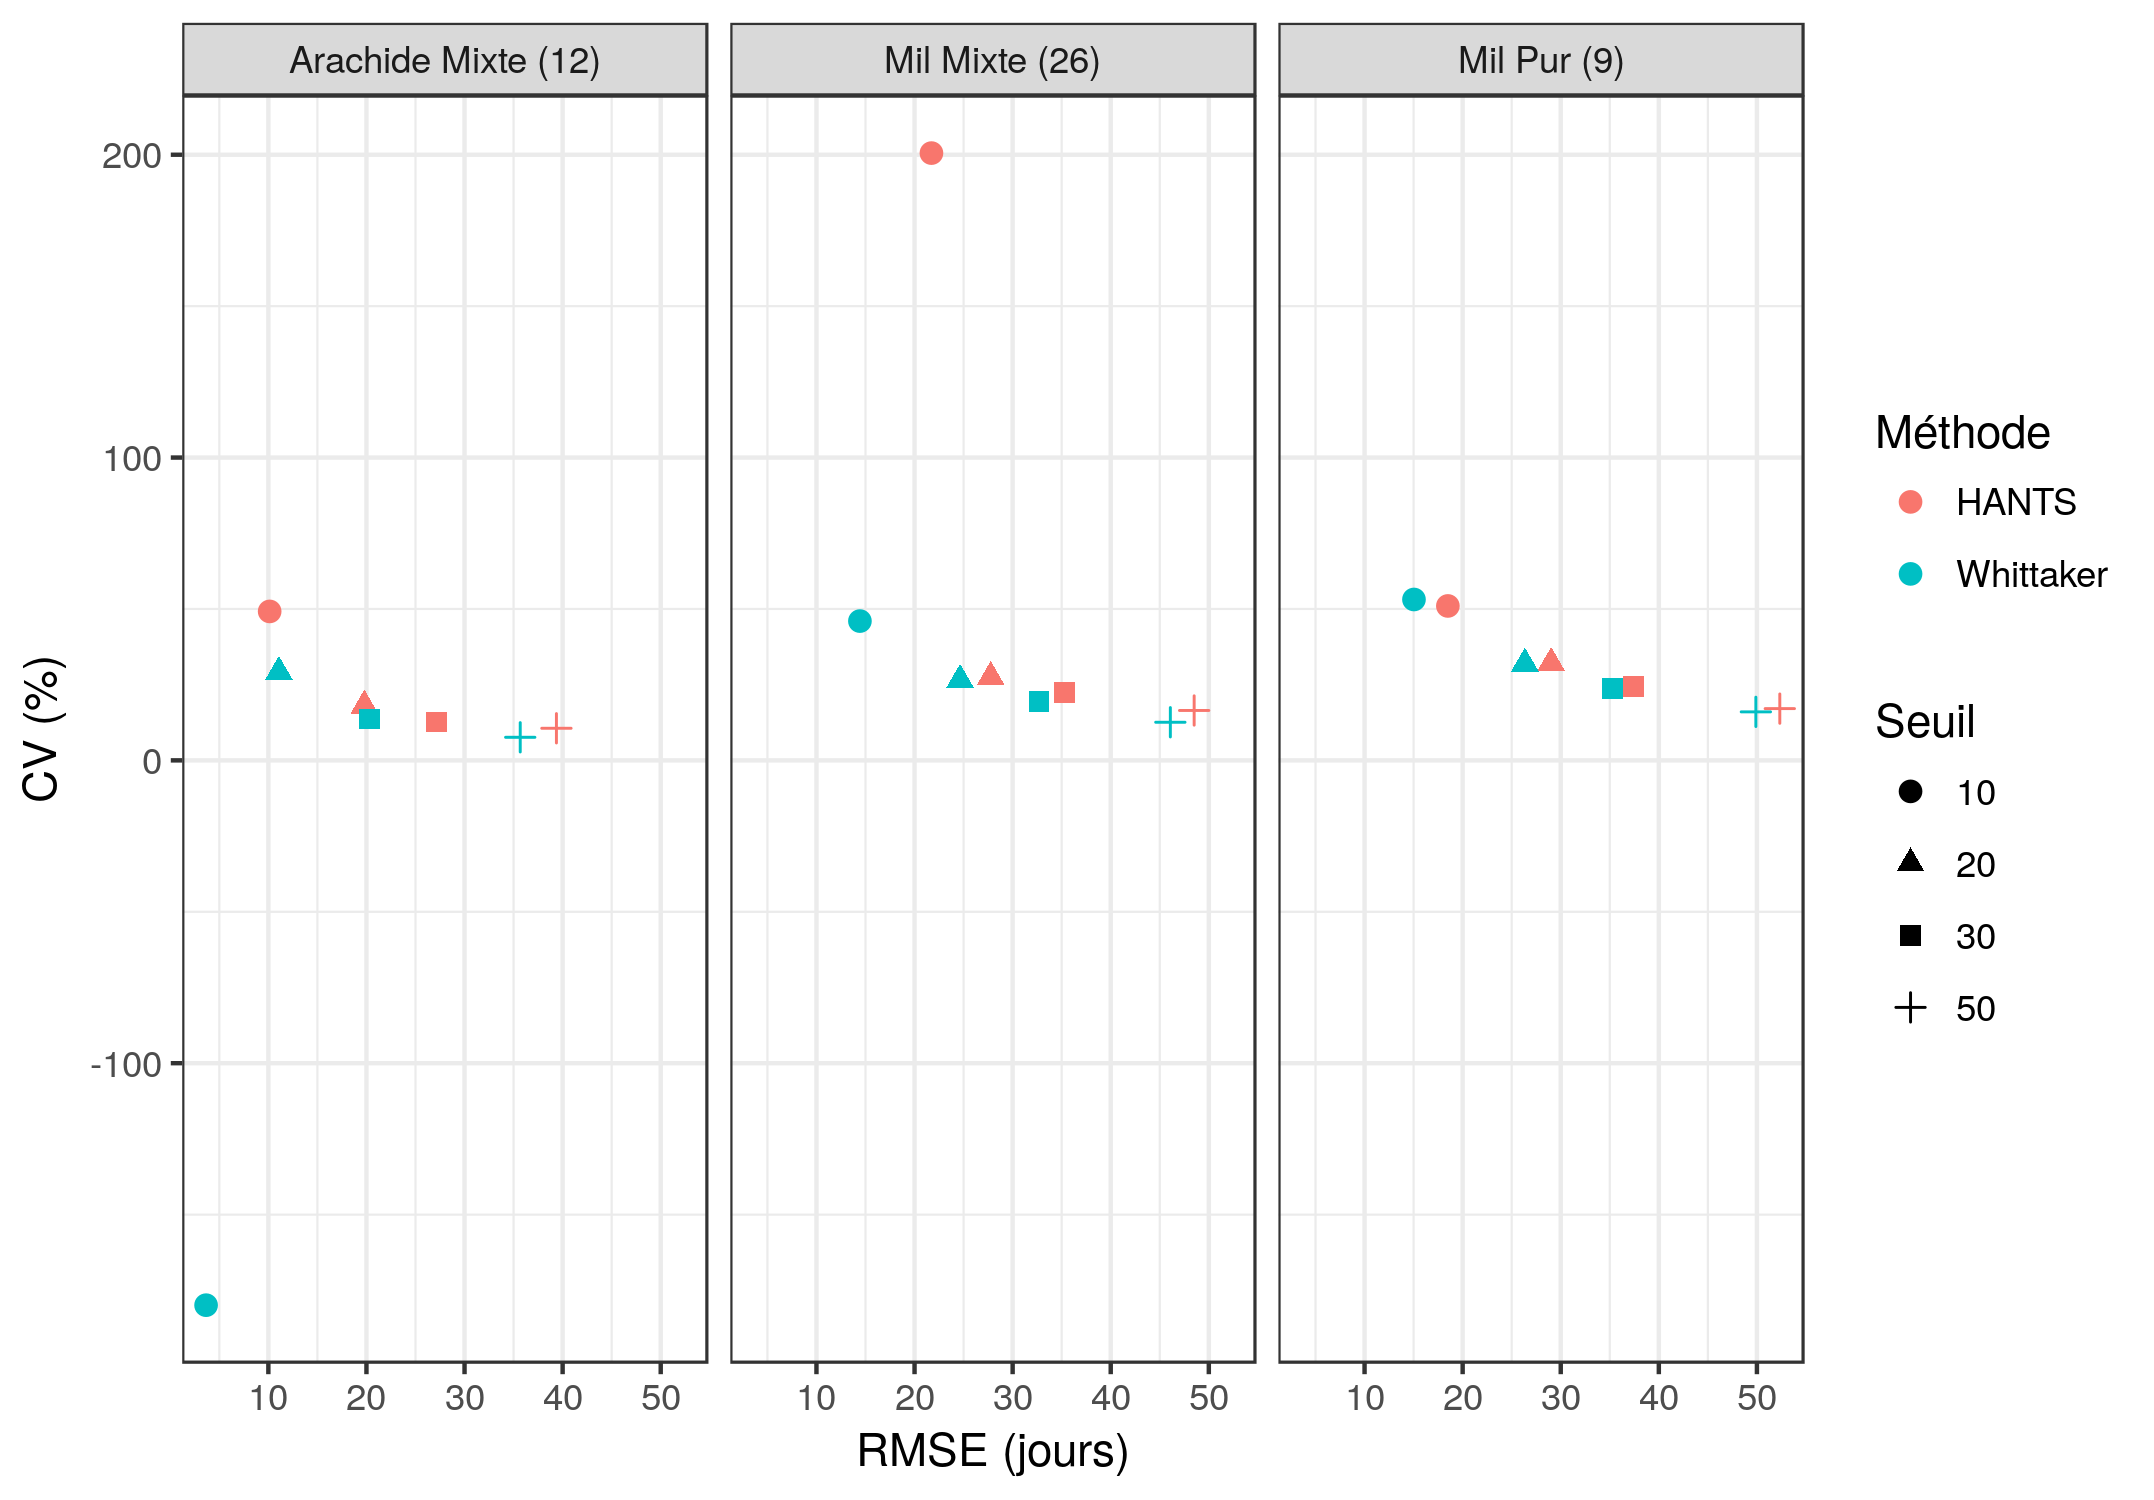
\includegraphics[scale=0.7]{resultats_discussions/SOS_RMSE_vs_CV.png} 
 \end{center}
 \caption[SOS -- RMSE vs CV]{Représentation du RMSE entre dates de semis et SOS estimés en fonction du coefficient de variation de leurs écarts par système de culture et méthode de lissage}
 \label{fig-sos-rmse-cv}
\end{figure}

\paragraph{EOS}

\subsection{Estimation des rendements}
  
\section{Discussions}

\subsection{Sur l'extraction du SOS et du EOS}

\subsection{Sur l'estimation des rendements}
